\section{Предикат поворота. Задача пересечения двух отрезков}

Даны два отрезка, которые задаются начальной и конечной точками $a, b \in \mathbb{R}^2$ и определяются как множества точек
$$ s = \{ (1-t)a + tb, t \in [0,1] \}. $$
Требуется проверить существование множества их общих точек. Для определения этого факта в вычислительной геометрии используется предикат \textit{левый поворот} (или по часовой стрелке). Рассмотрим возможные расположения точек и самих отрезков относительно друг друга:


\begin{figure}[h!]
	\centering
	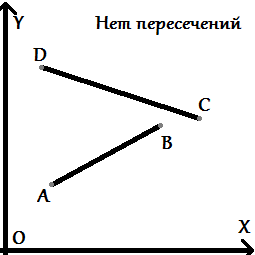
\includegraphics[width=0.4\linewidth]{img_easy/12_1.png}
	\captionsetup{labelformat=empty}
	\caption{}
\end{figure}

\textbf{Предикат <<левый поворот>>} --- выражение
$$
	\operatorname{LeftTurn}(a, b, c) =\left\{
	\begin{array}{rl}
		-1 &\mbox{, if}\ (c - a)\times(b - a) < 0\\
		0 &\mbox{, if}\ (c - a)\times(b - a) = 0\\
		1 &\mbox{, if}\ (c - a)\times(b - a) > 0
	\end{array}
	\right\}
$$

Определить, пересекаются ли два отрезка, можно с помощью предиката поворота. Ясно, что отрезки пересекаются тогда и только тогда, когда для каждого из отрезков его точки не лежат с одной стороны от второго отрезка. Пусть даны отрезки $a_0a_1$ и $b_0b_1$. Отрезки пересекаются, если

\begin{minted}{c}
	do_intersect = orientation(a0, a1, b0) != orientation(a0, a1, b1)
	and orientation(b0, b1, a0) != orientation(b0, b1, a1)	
\end{minted}

В случае, если обе ориентации в одной из строк равны нулю, отрезки лежат на одной прямой, и в этом случае пересечение можно проверить способом, аналогичным пересечению отрезков на действительной прямой (считаем, что точки сравниваются лексикографически):

\begin{minted}{c}
	between(x, a0, a1) = (a0 <= x <= a1)
	
	if a0 > a1
	    swap(a0, a1)
	
	if b0 > b1
	    swap(b0, b1)
	
	do_intersect = between(b0, a0, a1) || between(b1, a0, a1) ||
	               between(a0, b0, b1) || between(a1, b0, b1)
\end{minted}

Если предикат вычисления ориентации был абсолютно точным, то таким же будет описанный алгоритм.

